\documentclass[output=paper,colorlinks,citecolor=brown]{langscibook} 
%\bibliography{localbibliography}

\author{Pei-Jung Kuo\affiliation{National Chiayi University}}
\title{Three applicative GEIs in Mandarin Chinese}  
\abstract{This paper focuses on three types of applicative GEI distributed across three different syntactic layers in Mandarin Chinese. I propose that, in addition to \citegen{Tsai2017} high applicative GEI, which is located in the complementizer layer (above TP), there is also a differently behaved lower applicative GEI with two subtypes, one in the inflectional layer (between \textit{v}P and TP), and the other in the lexical layer (within \textit{v}P). This lower applicative GEI is shown to be different from other seemingly similar GEI PPs. Finally, a third kind of applicative GEI, also located in \textit{v}P, is presented and compared. The current study not only rounds out the distributional picture of applicative GEIs, but also provides us with more understanding of the lexical and syntactic diversity of GEI in Mandarin Chinese.}

\begin{document}
\SetupAffiliations{mark style=none}
\maketitle

\section{Introduction}\label{sec:kuo:1}
The lexical item \textit{gei} (`give/GEI') in Mandarin Chinese is well-known for its multiple functions. For example, it can function as a verb meaning `to give' in the double object construction in (\ref{kuo1}), and it can function as a preposition meaning `for' as in (\ref{kuo2}).


\ea
\label{kuo1}
\gll Zhangsan   gei-le              Lisi    yi-ben          shu.\\  
     Zhangsan   give-\textsc{asp}   Lisi    one-\textsc{cl} book\\ 
\glt `Zhangsan gave Lisi a book.'
\ex
\label{kuo2}
\gll Zhangsan   gei Lisi    xi      yifu.\\  
     Zhangsan   for Lisi    wash    cloth \\ 
\glt `Zhangsan washed clothes for Lisi.'
\z

Recently, \citet{Tsai2017} (see also \citealt{Tsai2012, Tsai2015b}) has proposed that \textit{gei} (`GEI') can also function as an applicative head with an affective reading in Mandarin Chinese, as shown in (\ref{kuo3}). 

\ea
\label{kuo3}
\gll Zhangsan   juran           gei wo  pao-le!\\  
     Zhangsan   unexpectedly    GEI me  run-\textsc{asp}\\ 
\glt `Zhangsan ran away on me unexpectedly!'
\z

Tsai observes that this applicative GEI is strictly speaker-oriented. Thus, an Affectee other than the first-person singular pronoun results in ungrammaticality, as shown in (\ref{kuo4}). In addition, he notes that the affective GEI-\textit{wo} phrase in a declarative sentence like (\ref{kuo5}) is awkward or unacceptable. Hence, an exclamatory force and evaluative mood are required for the applicative GEI in (\ref{kuo3}). In light of these requirements, Tsai proposes that GEI is an applicative head in an applicative projection located in the CP domain, which is associated with speaker attitudes.

{\judgewidth{??}
\ea[*]{
\label{kuo4}
\gll Zhangsan   juran           gei women/ni/nimen/ta/tamen    pao-le!\\  
     Zhangsan   unexpectedly    GEI us/you/you(\textsc{pl}.)/him/them   run-\textsc{asp}\\ 
\glt`Zhangsan ran away on us/you/you(pl.)/him/them unexpectedly!'
    }
\ex[??]{
\label{kuo5}
\gll Zuotian      Zhangsan    gei wo  pao-le.\\  
     yesterday    Zhangsan    GEI me  run-\textsc{asp}\\ 
\glt`Yesterday Zhangsan ran away on me.'
    }
\z}

In the following discussion, I will examine different types of applicative GEI located around the \textit{v}P periphery and will discuss their implications. In \sectref{sect2}, I argue that there is a GEI-\textit{wo} phrase lower than the affective GEI-\textit{wo} phrase in example (\ref{kuo3}), and that, despite appearing similar, it in fact behaves differently and has a distinct interpretation. In \sectref{sect3}, I further divide this lower GEI-\textit{wo} phrase into two subtypes. In \sectref{sect4}, I take a small detour to compare this lower GEI-\textit{wo} phrase with other confusing GEI-pronoun phrases/GEI PPs. In \sectref{sect5}, I present and compare an additional applicative GEI in \textit{v}P and discuss the distribution of applicative GEIs across syntactic layers in Chinese. I conclude this paper in the last section.

\section{A lower applicative GEI}\label{sect2}

In this section, I provide evidence that a lower GEI-\textit{wo} phrase is located around the \textit{v}P periphery and that it has a different denotation than the higher GEI-\textit{wo} phrase discussed by \citet{Tsai2017}. As mentioned in  \sectref{sec:kuo:1}, \citet{Tsai2017} has proposed a very high applicative GEI in the CP domain. Because of the
exclamatory force and evaluative mood associated with this GEI, he argues that it is located in an applicative projection above TP, and that an evaluative projection is also required to host the evaluative adverb \textit{juran} (`unexpectedly'). The derivational structure is shown in (\ref{kuo6}).

\ea
\label{kuo6}
\glt [\textsubscript{TopP} Zhangsan\textsubscript{i}  [\textsubscript{EvaP}   juran gei\textsubscript{j}  [\textsubscript{ApplP}  wo  t\textsubscript{j}  [\textsubscript{TP}  t\textsubscript{i}  ......]]]]\\  
\z

In structure (\ref{kuo6}), the applicative head GEI undergoes head movement to the head position of EvaP, the projection which also hosts the adverb \textit{juran} (`unexpectedly'). The Affectee \textit{wo} (`me') stays in the Spec, ApplP position, resulting in the correct word order of “GEI-\textit{wo}", and the subject in the Spec, TP position moves to the Spec, TopP position.
 
I would like to propose that, in addition to \possciteauthor{Tsai2017} (\citeyear{Tsai2017}) higher applicative GEI-\textit{wo} phrase in (\ref{kuo3}), a lower GEI-\textit{wo} phrase can also be found in Mandarin Chinese, as illustrated in example (\ref{kuo7}).

\ea
\label{kuo7}
\gll Ni     gei wo  guolai!\\  
     You    GEI me  come\\ 
\glt `You, come here!'
\z

At first glance, the lower applicative GEI appears similar to the one found in the higher domain. Note that, like the Affectee in the higher applicative GEI, the Affectee of this lower GEI can only be a first-person singular pronoun as shown in (\ref{kuo8}).

\ea[*]{
\label{kuo8}
\gll Ni     gei women/ni/nimen/ta/tamen     guolai!\\  
     You    GEI us/you/you(\textsc{pl}.)/him/them    come\\ 
\glt `*You, come here for us/you/him/them!'
    }
\z

However, despite this similarity, there are at least four differences between the lower GEI-\textit{wo} phrase in (\ref{kuo7}) and the higher GEI-\textit{wo} phrase in (\ref{kuo3}). First, while the higher GEI-\textit{wo} phrase needs an evaluative adverb in the sentence, the lower GEI-\textit{wo} phrase is incompatible with one, as shown in (\ref{kuo9}).

\ea[*]{
\label{kuo9}
\gll Ni     juran           gei wo  guolai!\\  
     you    unexpectedly    GEI me  come\\ 
\glt `*You, come here unexpectedly!'
    }
\z

Secondly, while the higher GEI-\textit{wo} phrase can have a second-person or third-person pronoun as the subject of the sentence, the lower GEI-\textit{wo} phrase can only have a second-person pronoun as the subject. This contrast is shown in (\ref{kuo10}) and (\ref{kuo11}), respectively.

\ea
\label{kuo10}
\gll Ni/Ta  juran           gei wo  pao-le!\\  
     You/he unexpectedly    GEI me  run-\textsc{asp}\\ 
\glt `You/He ran away on me unexpectedly!'
\ex
\label{kuo11}
\gll Ni/(*Ta)   gei wo  guolai!\\  
     You/he     GEI me  come\\ 
\glt `You/*He, come here!'
\z

Thirdly, recall that in example (\ref{kuo3}), the sentence containing the higher GEI-\textit{wo} phrase, the speaker is affected by (and is exclaiming at) the unexpected behavior of the subject. Hence, this higher GEI functions as an “affective-GEI". On the other hand, in example (\ref{kuo7}), the sentence with the lower GEI-\textit{wo} phrase, the speaker is making a forceful request/demand. In this case, the lower GEI could more aptly referred to as a ``demanding'' GEI.

Finally, when one utters sentence (\ref{kuo3}) containing the higher GEI-\textit{wo} phrase, the event denoted by this sentence has already been realized. The telic situation in example (\ref{kuo3}) thus contrasts with the atelic situation in the sentence containing a lower GEI-\textit{wo} phrase, where the event has not yet happened.

Based on the four contrasts above, it would appear that the ``demanding'' GEI-\textit{wo} phrase in (\ref{kuo7}) is distinct from the “affective" GEI-\textit{wo} phrase discussed in \citet{Tsai2017}. Note that the four characteristics of the demanding GEI-\textit{wo} phrase are bound tightly to its demanding denotation.\footnote{The generalization is also being pointed out by one of the reviewers.} Because of the demanding meaning, the evaluative adverb \textit{juran} is incompatible with the demanding GEI-\textit{wo} phrase. In addition, the demanding meaning is naturally co-related with an imperative sentence. And imperatives only allow second-person subjects. Furthermore, the forceful request interpretation is reminiscent of the demanding mood. Finally, when one makes a request/demand, it is also expected that the event denoted by the sentence has not be realized yet.

As for their respective syntactic positions, since the demanding GEI-\textit{wo} phrase is lower than the subject in (\ref{kuo7}), if the subject is in the standard subject position (Spec, TP), then we can infer that the GEI-\textit{wo} phrase is located in or below the TP domain, in contrast to the affective GEI-\textit{wo} phrase, which is located in the CP domain. The following two pieces of evidence indicate that the subject in (\ref{kuo7}) is in fact in the standard subject position (Spec, TP). First of all, \citet{Lin&Tang1995} propose that a true subject in Chinese can move to the matrix subject position with the raising modal \textit{yinggai} (`should'). And indeed the subject \textit{ni} (`you') in (\ref{kuo7}) can precede \textit{yinggai}, as shown in example (\ref{kuo12}).\footnote{The example without raising is shown in (\ref{kuoi}), as requested by one of the reviewers. A contrastive part is added in order to make this sentence more acceptable. 
\ea
\label{kuoi}
\gll    Yinggai	ni 	gei wo 	guolai, 	er 		bushi 	ta! \\ 
        should	you	GEI	me	come	rather	not		he\\
\glt    `You should come here, not him!'
\z
}

\ea
\label{kuo12}
\gll Ni     yinggai gei wo  guolai!\\  
     You    should  GEI me  come\\ 
\glt `You should come here!'
\z

Secondly, \citet{Li1990} has argued that the Chinese ECM verb \textit{yao} (`want') takes a TP as its complement. As shown in (\ref{kuo13}), example (\ref{kuo7}) can be the complement taken by the ECM verb \textit{yao} (`want'), which then indicates that the subject \textit{ni} (`you') is in the Spec, TP position. 

\ea
\label{kuo13}
\gll Wo yao     ni gei wo  guolai!\\  
     I  want    you GEI me  come\\ 
\glt `I want you to come here!'
\z

Based on the above observations, this new applicative GEI is indeed lower than the GEI in the CP domain in \citet{Tsai2017}. It has to be located in the TP domain, or lower, since the GEI-\textit{wo} phrase in (\ref{kuo7}) is lower than the subject in the Spec, TP position.

\section{Two positions}\label{sect3}

In the previous section, I proposed that the demanding GEI-\textit{wo} phrase is located in the TP domain, or lower. Here, I refer to relevant examples of the BA construction to argue more specifically that the demanding GEI is located around the \textit{v}P periphery, and that it has a higher and a lower subtype. The key example is shown in (\ref{kuo14}).

\ea
\label{kuo14}
\gll Ni     (gei wo)    ba  fangjian    (gei wo)    cao     ganjing!\\  
     you     GEI me     BA  room         GEI me     sweep   clean  \\ 
\glt `You, sweep and clean the room!'
\z

Example (\ref{kuo14}) is a BA construction, in which the object is preposed from a postverbal position to a preverbal BA NP position. In this example, the GEI-\textit{wo} phrase can be higher than BA or lower than the BA NP. \citet{Li2006} (see also \citealt{Haugnlili2009}) has proposed that BA is located in the head position of an independent \textit{Ba}P right above \textit{v}P, and that the BA NP is located in Spec, \textit{v}P. A typical BA construction and its structure is shown in (\ref{kuo15}).\footnote{The BA NP can be derived by movement or base-generation, see \citet{Li1&Thompson} for discussion. Here, I focus on the movement derivation.}

\ea
\label{kuo15}
  \ea{
  \gll Zhangsan	ba	shu		kan-wan-le.\\  
       Zhangsan	BA	book	read-finish-\textsc{asp}\\ 
  \glt `Zhangsan has finished reading the book.'
}
  \ex{
  \glt [\textsubscript{TP}  Zhangsan	[\textsubscript{BaP} ba	 [\textsubscript{\textit{v}P}  shu\textsubscript{i}		     [\textsubscript{VP}	 kan-wan-le  t\textsubscript{i} ]]]].\\
}
  \z
\z

Since the BA and the BA NP are located at the \textit{v}P periphery, they can be used as natural anchors to differentiate the syntactic positions of the two GEI-\textit{wo} phrases in (\ref{kuo14}). Let us focus on the GEI-\textit{wo} phrase higher than BA first. Because it is higher than BA but lower than the subject, \possciteauthor{kim2011} (\citeyear{kim2011, kim2012}) proposal that there is a peripheral applicative projection right above \textit{v}P comes to mind. Adopting this projection, the proposed structure for the GEI-\textit{wo} phrase between TP and \textit{v}P is shown in (\ref{kuo16}).

\ea
\label{kuo16}
\glt [\textsubscript{TP} Ni\textsubscript{i}  [\textsubscript{MP\textsubscript{Deo}}  gei\textsubscript{j}  [\textsubscript{peripheral ApplP}  wo  t\textsubscript{j}  [\textsubscript{\textit{v}P}  t\textsubscript{i}  ......]]]]\\  
\z

In structure (\ref{kuo16}), the applied NP \textit{wo} is base-generated at the specifier position of the peripheral applicative projection, and the applicative GEI undergoes head movement to the head position of a deontic modal projection. \citet{Tsai2015a} suggests the modal projection is right above \textit{v}P, as shown in (\ref{kuo17}).

\ea
\label{kuo17}
\glt [\textsubscript{TP} Subject\textsubscript{i}..... [\textsubscript{MP\textsubscript{Deo}}   Deontic modal  [\textsubscript{\textit{v}P}  t\textsubscript{i}  ......]]]\\  
\z

However, if it is instead above the peripheral applicative projection, its head position offers a natural landing site for the applicative GEI and could explain the ``demanding" mood of the GEI-\textit{wo} phrase, since the deontic modal is associated with a command or request mood.

For the GEI-\textit{wo} phrase that is lower than the BA NP, on the other hand, I draw on the high applicative of \citet{Pylkkanen2002, Pylkkanen2008}.\footnote{In addition to the high applicative, there is a contrastive low applicative. According to \citet{Pylkkanen2002}, transitivity and verb semantics diagnostics are the two primary ways to distinguish languages which contain a high applicative projection from languages which contain a low applicative projection. See \citet{Pylkkanen2002, Pylkkanen2008} for details and \sectref{sect5} of the current paper for discussion of \possciteauthor{Pylkkanen2002} low applicative.} This applicative is right above VP and denotes an applied relationship between an individual and an event. An example of \possciteauthor{Pylkkanen2008} high applicative projection and the simplified structure are shown in (\ref{kuo18}):

\ea
\label{kuo18}
    \ea[]{
    \langinfo{Luganda}{Bantu}{\citealt{Pylkkanen2002}: 25}\\
    \gll Mukasa ya-tambu-le-dde Katonga.\\  
         Mukasa \textsc{past}-walk-\textsc{appl}-\textsc{past} Katonga\\ 
    \glt `Muksasa walked for Katonga.'
}
    \ex[]{\label{kuo18b}
    \glt [\textsubscript{ApplHP} DP\textsubscript{Benefactive} [\textsubscript{ApplH'} Appl [\textsubscript{VP} V DP]]]
}
    \z
\z

Adopting the structure in (\ref{kuo18b}) for the GEI-\textit{wo} phrase lower than the BA NP, the applied NP \textit{wo} (`me') would be base-generated in the high applicative projection right above VP and would later move to the \textit{v} head position, as illustrated in (\ref{kuo19}).

\ea
\label{kuo19}
\glt [\textsubscript{TP} ..... [\textsubscript{\textit{v}P}   gei\textsubscript{i}  [\textsubscript{ApplHP}  wo    t\textsubscript{i}   [\textsubscript{VP} .....]]]]\\  
\z

Finally, since there is also a “demanding" mood exhibited in the sentence with this lower GEI-\textit{wo} phrase, I follow the proposal of \citet{Lin2001} that the \textit{v} head is a kind of light verb in Mandarin Chinese. Assuming that this light verb is a FOR-like light verb, the “demanding" meaning can be derived when the applicative GEI undergoes head movement to this light verb.\footnote{In \citet{Lin2001}, light verbs are proposed to be eventuality predicates with concrete thematic functions, and they are syntactic entities which can introduce arguments into the structure. In addition to the common ones such as \textsc{do}, \textsc{cause}, and \textsc{become}, other members include \textsc{exist}, \textsc{progress}, \textsc{at}, \textsc{use}, and \textsc{for} in Mandarin Chinese. An example of the \textsc{use} light verb is shown in (\ref{kuos}). The \textsc{use} light verb is located in the \textit{v} head position as in \REF{kuos1}, and it can be realized with a lexical light verb \textit{yong} (`with') as in \REF{kuos2}, or the main verb can raise to the \textit{v} head position as in \REF{kuos3}.
\ea
\label{kuos}
    \ea[]{
    \label{kuos1}
    \gll Ni     \textsc{use} na-ba   dao     qie,    wo  \textsc{use} zhe-ba  qie.    ~   (light verb \textsc{use})\\  
         you    ~   that-\textsc{cl} knife   cut     I   ~   this-\textsc{cl} cut\\ 
    \glt `You use this knife to cut, and I will use this one to cut.'
}
    \ex[]{
    \label{kuos2}
    \gll Ni     yong    na-ba   dao     qie,    wo  yong    zhe-ba  qie.  ~   (lexical light verb)\\  
         you    with   that-\textsc{cl}  knife   cut     I   with    this-\textsc{cl} cut\\ 
    \glt 
}
    \ex[]{
    \label{kuos3}
    \gll Ni     qie$_{\textnormal{j}}$+\textsc{use}  na-ba   dao     t$_{\textnormal{j}}$,   wo  qie$_{\textnormal{k}}$+\textsc{use}  zhe-ba  t$_{\textnormal{k}}$.  ~   (raising-to-\textit{v})\\  
         you    cut                     that-\textsc{cl} knife   ~                   I   cut                     this-\textsc{cl}\\ 
    \glt 
}
    \z
\z

Since the inventory of Chinese light verbs is still debatable (i.e. \citealt{Tsai2012}), here I simply assume that this For-like light verb can impose a forceful demand when GEI raises and incorporates with it. The exact nature of the For-like light verb is left for further research.}

To summarize, in this section I have shown that the demanding GEI-\textit{wo} phrase located around the \textit{v}P periphery has two subtypes -- one higher and one lower than \textit{v}P. In addition, like the derivation of the very high affective GEI-\textit{wo} phrase discussed by \citet{Tsai2017}, both subtypes of the demanding GEI-\textit{wo} phrase derive from the applicative GEI undergoing head movement to a higher functional projection. 

\section{Comparisons with other GEI-pronoun phrases}\label{sect4}

Before we proceed to further discussion of the demanding GEI-\textit{wo} phrase, in this section, I would like to compare the demanding GEI-\textit{wo} phrase with other confusing GEI-pronoun phrases.\footnote{The author would like to thank one of the reviewers who points out this potential issue.} As mentioned previously, GEI has multiple functions. Even if GEI is used as a preposition, it also has several interpretations. For example, the preposition GEI can introduce a receiver pronoun as in (\ref{kuoa}), a benefactive pronoun as in (\ref{kuob}), and a goal pronoun as in (\ref{kuoc}) (i.e. \citealt{Liu&Pan&Gu}). 

\ea
\label{kuoa}
\gll Ni     quai    gei baba    qian!\\  
     you    quickly GEI father  money\\ 
\glt `You, give Father money quickly!'
\ex
\label{kuob}
\gll Ni     quai    gei ta  jiejie  xinshang    de  geda!\\  
     you    quickly GEI he  solve   heart       DE  knot\\ 
\glt `You, solve the knot in his heart for him quickly!'
\ex
\label{kuoc}
\gll Ni     quai    gei tamen   jiang   ji-ge       gushi   ba!\\  
     you    quickly GEI them      tell    several-\textsc{cl}  story   \textsc{excl}\\ 
\glt `You, tell them several stories quickly!'
\z

In the above three examples, GEI also takes a pronoun to form a GEI-pronoun phrase, and they can be used in imperative forms. One may wonder how the demanding GEI-\textit{wo} phrase such as the one in (\ref{kuod}) can be distinguished from the above GEI-pronoun phrases when they both exhibit demanding interpretations.

\ea
\label{kuod}
\gll Bu     (gei wo)    ba zhe-quan di 	    (gei wo) chu-wan,   jiu bei 	xiang	chifan!\\  
     not    GEI me      BA this-\textsc{cl}  land    GEI me   hoe-finish JIU don't   think    eat   \\ 
\glt `Don't even think about eating if you do not finish hoeing the land!'
\z


According to what I have observed so far, I believe that there are at least three ways to tease these different GEIs apart. First of all, as discussed in (\ref{kuo8}) previously, the demanding GEI-\textit{wo} phrase only allows a first-person singular pronoun, as shown in (\ref{kuoh}). 

\ea
\label{kuoh}
\gll Ni     gei wo/*women/*ta/*tamem    guolai!\\  
     You    GEI me/us/him/them          come\\ 
\glt `You, come here (*for us/him/them)!'
\z

However, for other GEI-pronoun phrases, in addition to the first-person singular pronoun, they also allow first-person plural pronoun and third-person singular and plural pronouns, as shown from (\ref{kuol}) to (\ref{kuok}).\footnote{The second-person singular or plural pronoun has to be excluded here due to their pragmatic incompatibility with imperatives.}

\ea
\label{kuol}
\gll Ni     quai    gei wo/women/ta/tamen   qian!\\  
     you    quickly GEI me/us/him/them      money\\ 
\glt `You, give me/us/him/them money quickly!'
\ex
\label{kuoj}
\gll Ni     quai    gei wo/women/ta/tamen   jiejie  xinshang    de  geda!\\  
     you    quickly GEI me/us/him/them      solve   heart       DE  knot\\ 
\glt `You, solve the knot in the heart for me/us/him/them quickly!'
\ex
\label{kuok}
\gll Ni     quai    gei wo/women/ta/tamen   jiang   ji-ge       gushi   ba!\\  
     you    quickly GEI me/us/him/them      tell    several-\textsc{cl}  story   \textsc{excl}\\ 
\glt `You, tell me/us/him/them several stories quickly!'
\z

The above difference is because for the demanding GEI-\textit{wo} phrase, it is strictly speaker-oriented. But there is no such restriction for other GEI-pronoun phrases since the first-person/third-person pronouns, regardless singular or plural, can function as potential receivers, benefactives or goals.

Secondly, if one compares the interpretations of the four sentences from (\ref{kuoa}) to (\ref{kuod}), one can see that a crucial difference is that the demanding GEI-\textit{wo} phrase is entirely integrated into the sentence and the demanding mood is not translated at all. One can imagine the following scenario: When the speaker says something like (\ref{kuod}), the speaker can be part of the workers and he is simply the leader, who has to supervise the work. Hence these workers are not working for the speaker, and the speaker is not the receiver or goal of this action, either. The speaker's intention to say such a sentence (\ref{kuod}) is to tell the workers to work quicker. This is also the major reason why the GEI-\textit{wo} phrase cannot be translated at all in (\ref{kuod}), since for a sentence containing the GEI-\textit{wo} phrase, the GEI-\textit{wo} phrase simply functions as an emphatic marker to enforce the speaker's demanding order. However, for sentences from (\ref{kuoa}) to (\ref{kuoc}), the pronouns following GEI are interpreted as a receiver, a benefactive, or a goal. Therefore it is not possible to omit their existences and these GEI-pronoun phrases have to be translated fully as shown in the English translations.
 
Moreover, the different interpretations between the GEI-\textit{wo} phrase and the GEI-pronoun phrase can also be illustrated by synonymy substitution. Take the benefactive GEI-pronoun phrase for example. According to \citet{Liu&Pan&Gu}, when GEI introduces a benefactive, GEI can be replaced by \textit{wei} (`for') or \textit{ti} (`for'). Hence for example (\ref{kuob}), the GEI phrase can also be paraphrased with the WEI phrase or the TI phrase as in (\ref{kuoq}). After the substitution, the interpretation remains the same.

\ea
\label{kuoq}
\gll Ni     quai    gei/wei/ti ta  jiejie  xinshang    de  geda!\\  
     you    quickly GEI/WEI/TI he  solve   heart       DE  knot\\ 
\glt `You, solve the knot in his heart for him quickly!'
\z

However, if the demanding GEI-\textit{wo} phrase is replaced with the WEI phrase or the TI phrase as in (\ref{kuor}), the interpretation is different from the one in (\ref{kuod}). In example (\ref{kuor}), the pronoun \textit{wo} becomes a benefactive since it is introduced by WEI/TI. And this different interpretation can be clearly seen from the English translation.

\ea
\label{kuor}
\gll Bu (wei/ti wo) ba zhe-quan di      (wei/ti wo) chu-wan,   jiu bei 	    xiang   chifan!\\  
     not for/for me BA this-\textsc{cl}  land    for/for me  hoe-finish JIU don't    think   eat\\ 
\glt `Don't even think about eating if you do not finish hoeing the land for me!'
\z

Therefore we can conclude again that there indeed exist different interpretations between the demanding GEI-\textit{wo} phrase and other GEI-pronoun phrases.

Finally, we may expect different distributions between the demanding GEI-\textit{wo} phrase and other GEI-pronoun phrases according to their syntactic positions. In this paper, I have proposed that the demand GEI-\textit{wo} phrase do not form a constituent as in \sectref{sect3}. On the other hand, for other GEI-pronoun phrases, they are usually proposed to be PPs and adjoined to VP or \textit{v}P. Hence we can predict that it is not possible to have two demanding GEI-\textit{wo} phrases in the same syntactic position as in (\ref{kuom}), but it is possible to have two GEI-pronoun phrases in the same sentence since there can be several adjoined-PPs, as shown from (\ref{kuon}) to (\ref{kuop}).

\ea
\label{kuom}
\gll Bu     (gei wo)    (*gei wo)    ba zhe-quan di 	    chu-wan,   jiu bei 	xiang	chifan!\\  
     not     GEI me       GEI me     BA this-\textsc{cl}  land    hoe-finish JIU don't   think    eat   \\ 
\glt `Don't even think about eating if you do not finish hoeing the land!'
\ex
\label{kuon}
\gll Ni     quai    gei baba    gei mama    qian!\\  
     you    quickly GEI father  GEI mother  money\\ 
\glt `You, give Father and Mother money quickly!'
\ex
\label{kuoo}
\gll Ni     quai    gei ta  gei wo  jiejie  xinshang    de  geda!\\  
     you    quickly GEI he  GEI me  solve   heart       DE  knot\\ 
\glt `You, solve the knot in the heart for him and me quickly!'
\ex
\label{kuop}
\gll Ni     quai    gei tamen   gei women   jiang   ji-ge       gushi   ba!\\  
     you    quickly GEI them    GEI us      tell    several-\textsc{cl}  story   \textsc{excl}\\ 
\glt `You, tell them and us several stories quickly!'
\z

In addition, we can also predict that the demanding GEI-\textit{wo} phrase and other GEI-pronoun phrases should be able to co-occur in the same sentence once the context allows it. This predictions are borne out from (\ref{kuoe}) to (\ref{kuog}).

\ea
\label{kuoe}
\gll Ni     (gei wo)    quai    (gei wo)    gei baba    qian!\\  
     you     GEI me     quickly  GEI me     GEI father  money\\ 
\glt `You, give Father money quickly!'
\ex
\label{kuof}
\gll Ni     (gei wo)    quai    (gei wo)    gei ta  jiejie  xinshang    de  geda!\\  
     you     GEI me     quickly  GEI me     GEI he  solve   heart       DE  knot\\ 
\glt `You, solve the knot in his heart for him quickly!'
\ex
\label{kuog}
\gll Ni     (gei wo)    quai    (gei wo)    gei tamen   jiang   ji-ge       gushi   ba!\\  
     you     GEI me     quickly  GEI me     GEI them    tell    several-\textsc{cl}  story   \textsc{excl}\\ 
\glt `You, tell them several stories quickly!'
\z

In the above examples, there is a manner adverb \textit{quai} (`quickly'). Following \citet{Tsai2012}, manner adverbs in Mandarin Chinese adjoin to \textit{v}P. This then indicates that the two demanding GEI-\textit{wo} phrases can be higher or lower than \textit{v}P, as proposed above. Importantly, the co-occurrence of the demanding GEI-\textit{wo} phrase and other GEI-pronoun phrases points out that they are different types of GEI phrases syntactically.

To summarize, although there are other GEI-pronoun phrases and they seem to be quite similar to the demanding GEI-\textit{wo} phrase when these GEI phrases appear in imperative sentences, they do differ in their interpretations and syntactic distributions. Therefore, I believe the current proposal for the demanding GEI-\textit{wo} phrase can be maintained and can be distinguished from these GEI-pronoun phrases.

\section{Applicative GEIs in different layers}\label{sect5}

So far, we have seen that there are different applicative GEIs in Mandarin Chinese, and they are located in different syntactic domains. That is, the affective GEI-\textit{wo} phrase in \citet{Tsai2017} is in the CP domain, and the demanding GEI-\textit{wo} phrase under the current investigation which can be located in the TP or \textit{v}P domain. In this section, I would like to show that another type of applicative GEI can also be observed inside the \textit{v}P domain. Moreover, I suggest that the three types of applicative GEIs are distributed across the different syntactic layers proposed in \citet{Tsai2015a} for Chinese modals.

Employing the cartographic approach (i.e. \citealt{rizzi1997} and \citealt{cinque1999} and many others), \citet{Tsai2015a} proposes that the syntactic domains across which Chinese modals are distributed correspond to three syntactic layers, as is illustrated in \figref{kuo20}.

\begin{figure}
\caption{Chinese modals and their corresponding syntactic layers\label{kuo20}}
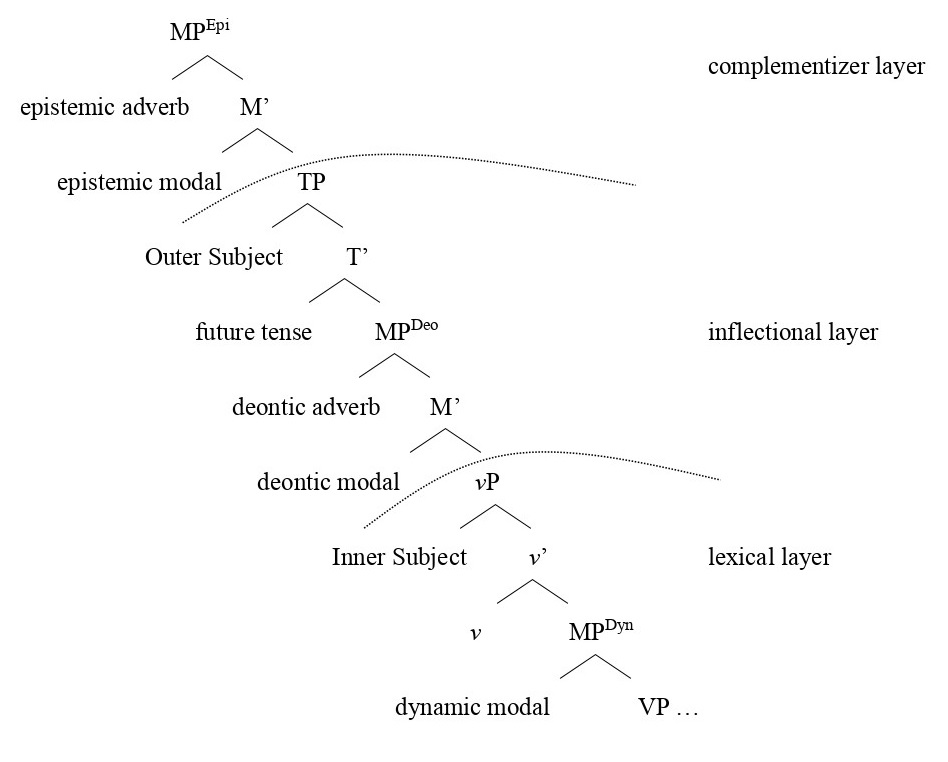
\includegraphics[align=t,width=11.5cm]{figures/tree2.jpg}
\end{figure}

In \figref{kuo20}, we can see that the epistemic modal is above TP in the complementizer layer; the deontic modal is between TP and \textit{v}P in the inflectional layer; and the dynamic modal is inside \textit{v}P in the lexical layer. The syntactic layer distribution can be simplified, as in (\ref{kuo21}), with TP and \textit{v}P viewed as layer boundaries.

\ea
\label{kuo21}
\glt    [ complementizer layer  [\textsubscript{TP}    inflectional layer  [\textsubscript{\textit{v}P}   lexical layer .....]]]\\  
\z

The distribution of three different kinds of modals in three syntactic layers is reminiscent of the distribution of applicative GEIs discussed thus far. Recall that the very high applicative GEI of  \citet{Tsai2017} is located in the CP domain and hence is in the complementizer layer. I have discussed a lower applicative GEI around the \textit{v}P periphery. Its subtypes above \textit{v}P and below \textit{v}P are located in the inflectional and lexical layer, respectively. In addition to occupying different layers, these applicative GEIs also have different denotations. The very high applicative GEI in \citet{Tsai2017} is an affective GEI, while the applicative GEI around the \textit{v}P periphery is a demanding GEI. In the following discussion, I present a distinct third kind of applicative GEI in Chinese. It is associated with a “transfer of possession" interpretation and can be observed in the lexical layer.

This ``transferring'' applicative GEI is found in double object constructions in Mandarin Chinese, a typical example of which is shown in (\ref{kuo22}).

\ea
\label{kuo22}
\gll Zhangsan   xie-gei-le              Lisi    yi-feng          xin.\\  
     Zhangsan   write-GEI-\textsc{asp}  Lisi    one-\textsc{cl} letter\\ 
\glt `Zhangsan wrote Lisi a letter.'
\z

In example (\ref{kuo22}), there is a transfer of possession of the letter from Zhangsan to Lisi. Note that the applicative GEI in example (\ref{kuo22}) is obligatory. Without it, the sentence is ungrammatical, as shown in example (\ref{kuo23}).\footnote{Note that it is not the case that all the double object constructions in Mandarin Chinese require an obligatory GEI. In \citet{Li1&Thompson}, they categorize double object constructions into three subtypes: the DOC without GEI, the DOC with an optional GEI, and the DOC with an obligatory GEI. See \citet{Li1&Thompson} for further discussion.}


\ea[*]{
\label{kuo23}
\gll Zhangsan   xie-le              Lisi    yi-feng          xin.\\  
     Zhangsan   write-\textsc{asp}  Lisi    one-\textsc{cl} letter\\ 
\glt intended: `Zhangsan wrote Lisi a letter.'
    }
\z

If GEI is an applicative GEI in example (\ref{kuo22}), the first applicative projection that comes to mind to host it is the lower applicative projection under \citet{Pylkkanen2002,Pylkkanen2008}. While \possciteauthor{Pylkkanen2002} high applicative projection is right above VP, her low applicative is in the complement position of the verb and denotes a transfer of possession between the applied NP and the direct object. An example of this low applicative projection and the simplified structure is shown in (\ref{kuo24}).

\ea
    \label{kuo24}
\ea[]{
    \langinfo{Japanese}{Altaic}{\citealt{Pylkkanen2002}: 24}\\
    \gll Taroo-ga Hanako-ni tegami-o kaita.\\  
         Taro-\textsc{nom} Hanako-\textsc{dat} letter-\textsc{acc} wrote\\ 
    \glt `Taro wrote Hanako a letter.'
}
    \ex[]{
    \glt [\textsubscript{VP} V [\textsubscript{ApplLP} DP\textsubscript{Goal} [\textsubscript{ApplL'} ApplL DP\textsubscript{Theme}]]]
}
    \z
\z

However, as pointed out by \citet{Paul&Whitman2010}, if the low applicative projection is adopted for example (\ref{kuo22}), the correct word order of the verb cluster cannot be derived, as shown in (\ref{kuo25}).

\ea[*]{
\label{kuo25}
\glt [\textsubscript{TP} Zhangsan [\textsubscript{AspP} gei-xie-le  [\textsubscript{VP} t\textsubscript{gei-xie}  [\textsubscript{ApplPL} Lisi  t\textsubscript{gei} yi-feng xin.]]]]\\  
    }
\z

Therefore, \citet{Paul&Whitman2010} propose a single applicative projection, which subsumes the functions of the high applicative and the low applicative of \citet{Pylkkanen2002, Pylkkanen2008}. As illustrated in example (\ref{kuo26}), when the applied NP is base-generated in Spec, ApplP, it functions like the applied Benefactive NP in \possciteauthor{Pylkkanen2002} (\citeyear{Pylkkanen2002, Pylkkanen2008}) high applicative structure. Paul and Whitman refer to the applicative in this context as the “thematic applicative." On the other hand, when the applied Goal NP raises from Spec, VP to Spec, ApplP, it functions like the applied Goal NP in \possciteauthor{Pylkkanen2002} (\citeyear{Pylkkanen2002, Pylkkanen2008}) low applicative structure. Paul and Whitman refer to the applicative in this context as the “raising applicative."

\ea
\label{kuo26}
    \ea
        \glt Thematic applicative\\
        \glt [\textsubscript{APPLP} DP\textsubscript{Benefactive} [\textsubscript{APPL'} Appl [\textsubscript{VP} V DP]]]
    \ex
        \glt Raising applicative\\
        \glt [\textsubscript{APPLP} DP\textsubscript{Goal} [\textsubscript{APPL'} Appl [\textsubscript{VP} t\textsubscript{Goal} [\textsubscript{V'} V DP\textsubscript{Theme} ]]]]
    \z
\z

In their \textit{raising applicative hypothesis}, \citet{Paul&Whitman2010} argue that the applicative projection should be above VP. Hence, the proposed structure for example (\ref{kuo22}) would be like that in (\ref{kuo27}).\footnote{For arguments that support this structure, readers are referred to \citet{Paul&Whitman2010} for details.} In this structure, the applied Goal NP is base-generated at Spec, VP and raises to Spec, ApplP. Importantly, the correct word order of the verb cluster can be derived under this proposal.

\ea
\label{kuo27}
\glt [\textsubscript{TP} Zhangsan [\textsubscript{AspP} xie-gei-le  [\textsubscript{ApplP}  Lisi [\textsubscript{Appl'} t\textsubscript{xie-gei} [\textsubscript{VP} t\textsubscript{Lisi}  [\textsubscript{V'} t\textsubscript{xie}  yi-feng          xin.]]]]]]\\  
\z

However, \citet{Kuo2016} has argued that, although the raised applied Goal NP is expected, the position of the ApplP in (\ref{kuo27}) may not be correct. For example, it is possible to have a high applicative projection and a low applicative projection appearing simultaneously in the same sentence. It would be hard to explain this phenomenon under the \textit{raising applicative hypothesis}. Thus, it seems that we do need two independent projections for the high applicative and the low applicative. Kuo adopts the light applicative projection of \citet{Citko2011}, which is right above VP and serves to host the raised Goal NP in languages such as Spanish and Polish. Note that this light applicative projection only functions as a landing site for the applied Goal NP, so \possciteauthor{Pylkkanen2002} (\citeyear{Pylkkanen2002, Pylkkanen2008}) low applicative projection is maintained under this system. The proposed structure is shown in \figref{kuo28}.

\begin{figure}
\caption{Chinese DOC structure proposed by \citet{Kuo2016}\label{kuo28}}
\begin{forest}
 [\textit{v}P
     [Zhangsan]
     [\textit{v}'
         [\textit{v}]
         [\ldots\ldots\\\textit{appl}P,align=center
             [Lisi\textsubscript{\textsc{goal}},name=goal]
             [\textit{appl}'
                 [GEI (\textit{appl})]
                 [VP
                     [write]
                     [ApplLP
                         [t,name=t]
                         [ApplL'
                             [ApplL]
                             [a letter\textsubscript{\textsc{theme}}]
                         ]
                     ]
                 ]
             ]
         ]
     ]
 ]
\draw [-{Triangle[]}] (t) to [bend left, looseness=1.25] (goal.225); 
\end{forest}
% % 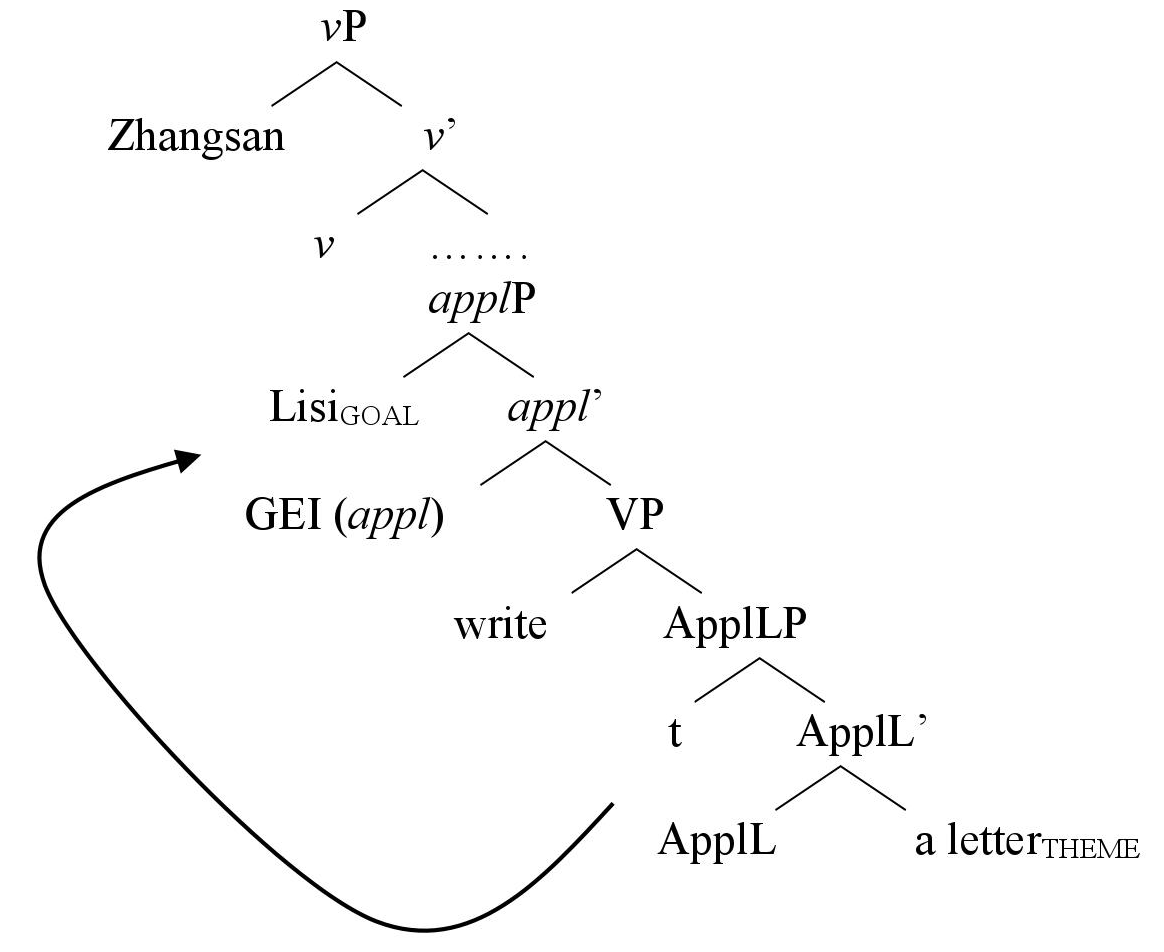
\includegraphics[width=9cm]{figures/tree.png}
\end{figure}

In \figref{kuo28}, the main verb \textit{xie} (`write') undergoes head movement and incorporates with GEI on its way to the \textit{v} head, and the correct word order of the verb cluster can be derived. Moreover, since the Goal NP moves from Spec, ApplLP to Spec, light applP, the correct position of the Goal NP can also be derived via raising to this higher position.\footnote{Both reviewers wonder why the transferring GEI cannot be the realization of the \textit{v} head directly. The fact that the transferring GEI has to be base-generated lower than the \textit{v} head can be seen from the following BA construction with an optional emphatic \textit{gei} (`GEI').

\ea
\label{kuoii}
\gll Zhangsan ba zhe-feng	xin (gei)	xie-gei-le 		Lisi.\\
Zhangsan \textsc{ba} this-\textsc{cl} letter	\textsc{gei}	write-\textsc{gei}-\textsc{asp}	Lisi
\\
\glt `Zhangsan wrote this letter to Lisi.'
\z

Available in the BEI construction (Chinese passive construction) as well, \citet{Tang2001} has proposed that this optional emphatic GEI can function as a marker of affectedness, which is a head located in a functional projection XP right above VP. (This XP proposal is reminiscent of the high applicative projection by \citet{Pylkkanen2002, Pylkkanen2008}). Since the verb cluster containing the transferring GEI in (\ref{kuoii}) has to be lower than this optional emphatic GEI, it is therefore not possible for the transferring GEI to be a direct realization of the \textit{v} head.}


%\footnote{Both reviewers wonder why the transferring GEI cannot be the realization of the \textit{v} head directly and has to be the lower applicative head. The fact that the transferring GEI has to be lower than the \textit{v} head can be seen from the following sentence containing the BA phrase. 
%\ea
%\label{kuoii}
%\gll Zhangsan ba zhe-feng xin xie-gei-le Lisi.\\ 
%     Zhangsan BA this-CL letter write-GEI-ASP Lisi\\
%\glt 'Zhangsan wrote this letter to Lisi.'
%\z
%As mentioned previously, BA in the BA phrase is proposed to be located in the \textit{v} head. Hence in example (\ref{kuoii}), the transferring GEI can only be base-generated lower than BA in order to form a verb cluster with the main verb. This example therefore shows that the transferring GEI cannot be a direct realization of the \textit{v} head.}

To summarize, in this section I have discussed another kind of applicative GEI in the \textit{v}P domain. This applicative GEI is associated with a ``transfer of possession'' interpretation and involves low and light applicative projections. All the applicative GEIs we have examined so far are summarized in Table \ref{kuotab:1:three}.

\begin{table}
\caption{Summary of applicative GEIs}
\label{kuotab:1:three}
 \begin{tabular}{lllll} 
  \lsptoprule
            & GEI1 & GEI2 & GEI 2 & GEI3\\ 
  \midrule
  denotation  &  affective &  demanding &  demanding  & transferring\\
  syntactic position  & CP & TP & \textit{v}P & \textit{v}P\\
  \lspbottomrule
 \end{tabular}
\end{table}

In Table \ref{kuotab:1:three}, there are three different kinds of GEI, referred to as GEI1, GEI2, and GEI3, respectively. The first GEI is an affective applicative GEI, as argued in \citet{Tsai2017}, and it is located in the CP domain. The second GEI is a demanding applicative GEI, which can be found in the TP or \textit{v}P domains. The last GEI is a transferring applicative GEI, which has been discussed in \citet{Paul&Whitman2010} and \citet{Kuo2016}. This transferring GEI is also located in the \textit{v}P domain. By utilizing \possciteauthor{Tsai2015b} (\citeyear{Tsai2015a}) syntactic layer proposal for Chinese modals, I have shown that different applicative GEIs can also be found in three different syntactic layers.

\section{Conclusion}\label{sect6}

In this paper, I have discussed various applicative GEIs in Mandarin Chinese and their different syntactic distributions. What we have observed thus far has interesting implications for the theory of syntactic layers. Recall that \citet{Tsai2017} has proposed three different syntactic layers in Mandarin Chinese to account for the distribution of Chinese modals. In addition, he argues that the verb GEI in example (\ref{kuo1}), the preposition GEI in example (\ref{kuo2}), and the applicative GEI in example (\ref{kuo3}) also occupy these same syntactic layers, as summarized in Table \ref{kuotab:2:different}.

\begin{table}
\caption{\citet{Tsai2017}}
\label{kuotab:2:different}
 \begin{tabular}{lllll} 
  \lsptoprule
            & affective GEI & benefactive GEI & giving GEI\\ 
  \midrule
  form  &   applicative &    preposition  &   verb\\
  domain & CP & TP & \textit{v}P\\
  syntactic layer  & complementizer & inflectional & lexical\\
  \lspbottomrule
 \end{tabular}
\end{table}

He further proposes that these different forms of GEI follow a grammaticalization track from the bottom to the top syntactic layers, with the verb GEI in the lexical layer developing into a preposition in the inflectional layer, and then later into a high applicative head in the complementizer layer. 
 
While \citet{Tsai2017} focuses on different syntactic categories and their distribution across the three layers, I show that different types of applicative GEI are similarly distributed, each correlating with a specific function/interpretation, as shown in Table \ref{kuotab:3:different2}.

\begin{table}
\caption{Applicative GEIs}
\label{kuotab:3:different2}
 \begin{tabular}{lllll} 
  \lsptoprule
            & Applicative GEI1 & Applicative GEI2 & Applicative GEI3\\ 
  \midrule
  function & affective & demanding & transferring\\
  domain & CP & TP & \textit{v}P\\
  syntactic layer  & complementizer & inflectional & lexical\\
  \lspbottomrule
 \end{tabular}
\end{table}

I draw on \possciteauthor{Tsai2017} (\citeyear{Tsai2017}) analysis of the high affective GEI in the complementizer layer, a layer which has many discourse-related projections, and add to the discussion by proposing a “demanding" GEI in the inflectional layer, the location of the deontic modal with its associated command/request mood. Further, I suggest there is a lower “transferring" GEI, which, like the verb GEI, is associated with a giving action and occupies the lexical layer. In conclusion, these two studies of GEI not only enable us to understand more about the multi-functions of GEI in Mandarin Chinese, but also help to expand the investigation of applicative systems and syntactic layers more generally.

\section*{Acknowledgments}
This paper is part of my research sponsored by the Ministry of Science and Technology, Taiwan (Grant No. MOST 108-2410-H-415-001). I hereby acknowledge the financial support of the MOST. I would also like to thank the two anonymous reviewers for their valuable comments and suggestions on the previous version of this paper. All errors remain mine.


\section*{Abbreviations}
\begin{multicols}{2}
\begin{tabbing}
AppLHP\hspace{1ex}\=High applicative projection\kill
ACC \> Accusative\\ 
APPL \> Applicative\\ 
ApplHP \> High applicative projection\\ 
ApplLP \> Low applicative projection\\
ASP \> Aspect marker\\ 
CL \> Classifier\\
DAT \> Dative\\
Deo \> Deontic\\
Dyn \> Dynamic\\ 
Epi \> Epistemic\\
EvaP \> Evaluative projection\\ 
MP \> Modal projection\\ 
NOM \> Nominative\\ 
PAST \> Past tense\\ 
TopP \> Topic projection
\end{tabbing}
\end{multicols}

{\sloppy\printbibliography[heading=subbibliography,notkeyword=this]}
\end{document}
